\documentclass{article}

\usepackage{mathtools}
\usepackage[margin=1.5in]{geometry}
\usepackage{float}
\usepackage{verbatim}
\usepackage{graphicx}
\usepackage{amsthm}
\usepackage{xfrac}
\usepackage{tikz} % oh ho...
%\usepackage{svg} % I gave up...

\restylefloat{table}

\author{Guillaume Labranche (260585371)}
\title{COMP 531 -- Advanced Theory of Computation\\Assignment \#2}
\date{due on 10 February 2016}

\newcommand{\R}{\mathbb{R}}
\newcommand{\F}{\mathbb{F}}
%\newcommand{-->}{\rightarrow} %does not work :(
\newtheorem{theorem}{Theorem}
\newtheorem{corollary}{Corollary}
\newtheorem{lemma}{Lemma}
\newtheorem{proposition}{Proposition}

\begin{document}

\pagenumbering{gobble}
\maketitle

\begin{enumerate}

\item Here we assume that by log-space computable functions, we mean functions which can be computed by a log-space transducer, that is a TM with a read-only input tape, a log-space bounded work tape and a write-only output tape.

\begin{proof} In the trivial solution, for any input $x$ to $f \circ\ g$, we first compute $g(x)$ and then run $f$ on $g(x)$'s output tape. Let $n=|x|$. While $g(x)$ requires logarithmic work space, its output may be polynomial. Let $n' = |g(x)| = O(n^k)$. Then $f(g(x))$ requires $O(\log(n^k)) = O(k \log n) = O(\log n)$ work space. Although individually $f$ and $g$ only require logarithmic space, storing $g(x)$ requires polynomial space. Therefore we devise a trick that enables us to compute $f(g(x))$ without storing $g(x)$.

We modify the transducer $F$ for computing $f$ as follows. Whenever $F$ reads the $i$th symbol of its input tape (which contains $g(x)$), it runs the transducer $G$ for $g$ on $x$ until the $i$th symbol is outputted (transducers have a write-only output tape). This can be done using two counters of size $O(\log(n^k))=O(\log n)$ each, one for storing the position on $F$'s input tape and one for keeping track of the number of symbols outputted by $G$. As we can see, $f \circ g$ is still computable in logarithmic space because we do not store $g(x)$, only one character at a time and two counters of logarithmic size.
\end{proof}

\newpage
\item \begin{theorem}This algorithm detects a cycle $\iff$ there is a cycle.\end{theorem}
\begin{proof}
($\implies$) Consider the only way that the algorithm detects a cycle: When the son is placed at a vertex $v$, leaves through an edge $(v,u)$ and comes back to $v$ through a different edge $(w,v)$ where $u\not=w$. In this case, there is a path from $v$ to $u$, from $u$ to $w$ and from $w$ to $v$. This forms a cycle.

($\Longleftarrow$) When following edge $(v,u)$, the son following the ``cycle searching principle'' always visits all the neighbours of $u$ in sequential order before going back through $(u,v)$. Therefore if the node $v$ is the root of a tree (acyclic graph) the son will perform a tree traversal, coming back along an edge only if the subtree has been been entirely visited. In the case that there is a cycle containing $v$, $u$ and $w$ where $(v,u),(v,w)\in E$, the son will eventually be brought to $v$ by his father. The son will leave $v$ through the edge $(v,u)$ and eventually reach $w$. At that point he will re-enter $v$ and the cycle will be detected.
\end{proof}
\begin{theorem}This algorithm terminates in finite time.\end{theorem}
\begin{proof} (by contradiction) The algorithm evaluates the following condition:

$\forall v\in V, \forall (v,u)\in E$, the son follows $(v,u)$ and comes back to $v$ through $(u,v)$. Since $V$ and $E$ are finite, the only way for the algorithm to not be able to evaluate the condition is if the son does not ever come back to $v$. By the pigeonhole principle, since $V$ is finite the son must follow one edge more than once. The son's behaviour at a particular vertex $v$ is solely dependant on the previous visited vertex and the edges of $v$. Since $G$ does not change during the algorithm's runtime, visiting the same edge in the same direction twice will lead to the exact same behaviour and the son will be stuck in a loop. We will show that such a loop cannot exist.

Let $s\in V$ be a vertex where the son was taken to by his father. Assume that there is a loop in the path taken by the son and let $(w,z)\in E$ be the first edge that he visits twice in his path $P=(s,\dotsc,u,w,z,\dotsc,v,w,z,\dotsc)$. Let $(u,w)$ be the $i$th edge of $w$. The index of $(w,z)$ is $i+1$, as per the algorithm description. In the second occurence of $(w,z)$, the son follows the $(i+1)$th edge of $w$. This means that it entered $w$ through $w$'s $i$th edge. Therefore $u=v$ and $(u,w)=(v,w)$ is a repeated edge visited before $(w,z)$, which contradicts our assumption. Therefore there cannot be such a loop in his path and he will eventually return to $s$.
%When entering a vertex $u$ of fanout $k$, the son will follow edges $(i+1,i+1,$
%When following the edge $(v,u)$, the son follows all other edges of $u$ before coming back through $(v,u)$. 
%The son traverses the graph following the ``cycle searching principle'', starting at every vertex once. Therefore I will show that this principle terminates 
\end{proof}

The algorithm only needs to store a constant amount of vertex indexes:
\begin{itemize}
\item which vertex the father is visiting
\item which vertex the son visits initially
\item which vertex the son last visited while traversing the graph
\end{itemize}
Therefore the space complexity is $O(\log |V|)$.

\newpage
\item First we note that the description of a symmetric boolean function $f:\{0,1\}^n\rightarrow \{0,1\}$ is basically a mapping $m:\{0,1,\cdots,n\}\rightarrow \{0,1\}$.


Next, we introduce a new type of gate MAJ$_{\geq i}$ constructed from a single MAJ gate that returns 1 when $i$ or more of its $n$ input wires are turned on, and 0 otherwise. To construct it, we feed all $n$ inputs into a MAJ gate. We also add $i-1$ 0-constant inputs and $n-i$ 1-constant inputs for a total of $2n-1$ inputs. Therefore the MAJ gate will output 1 when:
\begin{align*}
\#_1 &> \frac{2n-1}{2} \\
\#_1 &\geq n \\
\#_1 &\geq i + (n-i \text{ 1-constants}) \\
\#_1 &\geq i \text{ [since the constants are fixed once gate is built]}
\end{align*}
The following diagram illustrates the strategy visually:

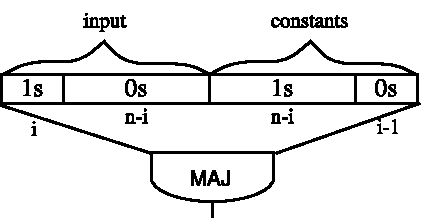
\includegraphics{q3_maj_geq.pdf}

\begin{comment}
Its construction is divided in two cases:
\begin{itemize}
\item $i \geq \sfrac{n}{2}$: We simply feed all $n$ inputs into a MAJ gate and add 0-constant inputs until the gate has $2i-1$ inputs. The gate will output 1 when: 
\begin{align*}
\#_1 &> \frac{2i-1}{2} \\
\#_1 &\geq i
\end{align*}
where $\#_1$ denotes the number of non-constant inputs (i.e. the one that matter) into the gate with value 1.
\item $i < \sfrac{n}{2}$: 
\end{itemize}
\end{comment}

We also introduce a similar gate MAJ$_{\leq i}$ that returns 1 if $i$ or less inputs are turned on and 0 otherwise. Its construction is very similar to MAJ$_{\geq i}$ but with negated inputs. Checking whether there are at most $i$ 1s is equivalent to checking whether there are more than $n-i$ 0s. Thus we negate all $n$ inputs and feed them into a MAJ gate. We then add $n-i$ 0-constant inputs and $i+1$ 1-constant inputs so that the MAJ gate has fanin $2n+1$. Therefore the MAJ gate will output 1 when:
\begin{align*}
\#_1 &> \frac{2n+1}{2} \\
\#_1 &> n + \sfrac{1}{2} \\
\#_1 &> n + \\
\#_0 &\leq n \\ 
\#_0 &\leq i + (n-i \text{ 0-constants})
\end{align*}
Since we negated the $n$ inputs, this is equivalent to checking that $$\#_1(\text{original input}) \leq i$$

We then introduce a new type of gate EQ$_i:\{0,1\}^n\rightarrow\{0,1\}\times\{0,1\}$ composed of a MAJ$_{\geq i}$ and a MAJ$_{\leq i}$. On input $w$, it will output $1 \times 1$ if $\#_1(w)=i$, and $1 \times 0$ if $\#_1(w)\not=i$.

Now to construct a circuit to compute $f$, for all $i$ such that $f(i)=1$, add an EQ$_i$ gate with the same inputs as $f$ at level 1.  At level 2, add a single MAJ gate taking all our level 1 gates as input.

In order to show that this indeed computes $f$, let's perform a case analysis on $f(j)$ for all $0\leq j \leq n$:
\begin{itemize}
\item $f(j)=1$: This will make all the EQ$_{i\not=j}$ return $1 \times 0$ or $0 \times 1$ except the gate EQ$_{i=j}$ which will return $1 \times 1$. There will be more 1s than 0s feeding into the level 2 MAJ gate and the circuit will output 1.

\item $f(j)=0$: This will result in all EQ gates returning $1 \times 0$ or $0 \times 1$ since no EQ$_{i=j}$ gate has been added to the circuit. Therefore the number of 0s and 1s will be equal and the level 2 MAJ gate will output 0.

\end{itemize}

\newpage
\item %todo

\newpage
\item %todo

\end{enumerate}
\end{document}
